% !TeX spellcheck = en_GB
% !TeX root = ../phd-thesis.tex

\begin{figure*}
    \centering
    \def\astscale{0.38}
    \begin{subfigure}[]{0.25\linewidth}
        \centering
        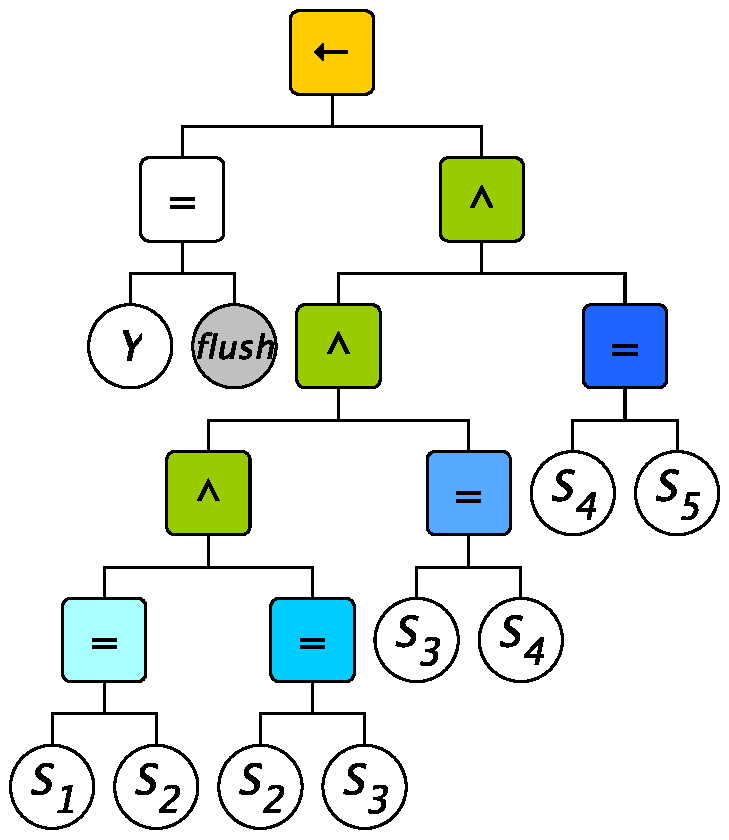
\includegraphics[width=\linewidth]{figures/ast-flush-1.pdf}
        \caption{AST of a formula}
        \label{fig:ast-kins-unencoded}
    \end{subfigure}
    \hfill$\rightarrow$\hfill
    \begin{subfigure}[]{0.32\linewidth}
        \centering
        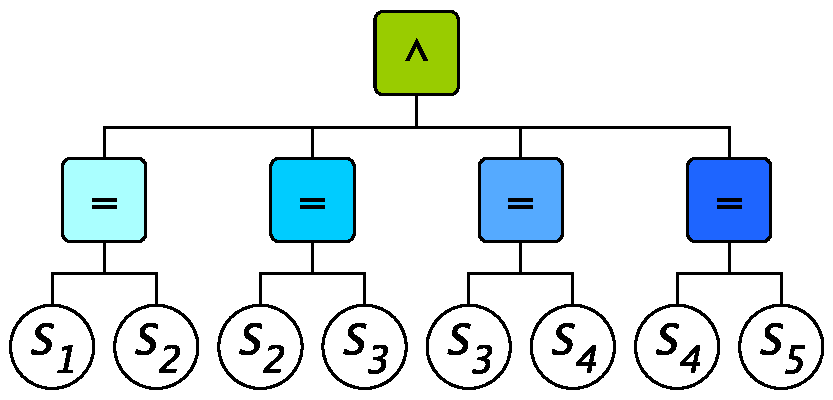
\includegraphics[width=\linewidth]{figures/ast-flush-2.pdf}
        \caption{Optimised AST of a formula}
        \label{fig:ast-kins-optimised}
    \end{subfigure}
    \hfill$\rightarrow$\hfill
    \begin{subfigure}[]{0.35\linewidth}
        \centering
        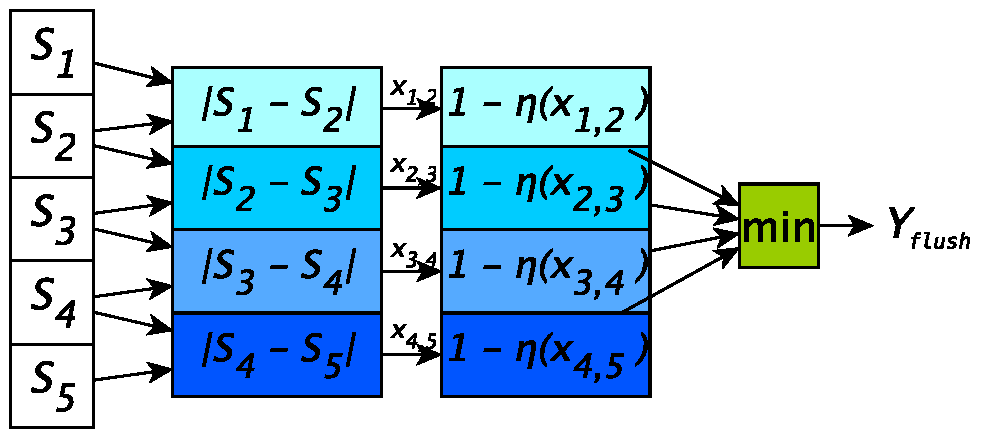
\includegraphics[width=\linewidth]{figures/net-flush.pdf}
        \caption{Layers from the optimised AST}
        \label{fig:net-kins-encoded}
    \end{subfigure}
    \caption{
        Example of the encoding process of formulas into module network.
        %
        Box coloured in the same way represent the encoding of a given operator through each encoding step.
    }
    \label{fig:ast-kins}
\end{figure*}
